\PassOptionsToPackage{unicode=true}{hyperref} % options for packages loaded elsewhere
\PassOptionsToPackage{hyphens}{url}
%
\documentclass[]{article}
\usepackage{lmodern}
\usepackage{amssymb,amsmath}
\usepackage{ifxetex,ifluatex}
\usepackage{fixltx2e} % provides \textsubscript
\ifnum 0\ifxetex 1\fi\ifluatex 1\fi=0 % if pdftex
  \usepackage[T1]{fontenc}
  \usepackage[utf8]{inputenc}
  \usepackage{textcomp} % provides euro and other symbols
\else % if luatex or xelatex
  \usepackage{unicode-math}
  \defaultfontfeatures{Ligatures=TeX,Scale=MatchLowercase}
\fi
% use upquote if available, for straight quotes in verbatim environments
\IfFileExists{upquote.sty}{\usepackage{upquote}}{}
% use microtype if available
\IfFileExists{microtype.sty}{%
\usepackage[]{microtype}
\UseMicrotypeSet[protrusion]{basicmath} % disable protrusion for tt fonts
}{}
\IfFileExists{parskip.sty}{%
\usepackage{parskip}
}{% else
\setlength{\parindent}{0pt}
\setlength{\parskip}{6pt plus 2pt minus 1pt}
}
\usepackage{hyperref}
\hypersetup{
            pdftitle={Assignment 1},
            pdfauthor={Michal Malyska},
            pdfborder={0 0 0},
            breaklinks=true}
\urlstyle{same}  % don't use monospace font for urls
\usepackage[margin=1in]{geometry}
\usepackage{color}
\usepackage{fancyvrb}
\newcommand{\VerbBar}{|}
\newcommand{\VERB}{\Verb[commandchars=\\\{\}]}
\DefineVerbatimEnvironment{Highlighting}{Verbatim}{commandchars=\\\{\}}
% Add ',fontsize=\small' for more characters per line
\usepackage{framed}
\definecolor{shadecolor}{RGB}{248,248,248}
\newenvironment{Shaded}{\begin{snugshade}}{\end{snugshade}}
\newcommand{\AlertTok}[1]{\textcolor[rgb]{0.94,0.16,0.16}{#1}}
\newcommand{\AnnotationTok}[1]{\textcolor[rgb]{0.56,0.35,0.01}{\textbf{\textit{#1}}}}
\newcommand{\AttributeTok}[1]{\textcolor[rgb]{0.77,0.63,0.00}{#1}}
\newcommand{\BaseNTok}[1]{\textcolor[rgb]{0.00,0.00,0.81}{#1}}
\newcommand{\BuiltInTok}[1]{#1}
\newcommand{\CharTok}[1]{\textcolor[rgb]{0.31,0.60,0.02}{#1}}
\newcommand{\CommentTok}[1]{\textcolor[rgb]{0.56,0.35,0.01}{\textit{#1}}}
\newcommand{\CommentVarTok}[1]{\textcolor[rgb]{0.56,0.35,0.01}{\textbf{\textit{#1}}}}
\newcommand{\ConstantTok}[1]{\textcolor[rgb]{0.00,0.00,0.00}{#1}}
\newcommand{\ControlFlowTok}[1]{\textcolor[rgb]{0.13,0.29,0.53}{\textbf{#1}}}
\newcommand{\DataTypeTok}[1]{\textcolor[rgb]{0.13,0.29,0.53}{#1}}
\newcommand{\DecValTok}[1]{\textcolor[rgb]{0.00,0.00,0.81}{#1}}
\newcommand{\DocumentationTok}[1]{\textcolor[rgb]{0.56,0.35,0.01}{\textbf{\textit{#1}}}}
\newcommand{\ErrorTok}[1]{\textcolor[rgb]{0.64,0.00,0.00}{\textbf{#1}}}
\newcommand{\ExtensionTok}[1]{#1}
\newcommand{\FloatTok}[1]{\textcolor[rgb]{0.00,0.00,0.81}{#1}}
\newcommand{\FunctionTok}[1]{\textcolor[rgb]{0.00,0.00,0.00}{#1}}
\newcommand{\ImportTok}[1]{#1}
\newcommand{\InformationTok}[1]{\textcolor[rgb]{0.56,0.35,0.01}{\textbf{\textit{#1}}}}
\newcommand{\KeywordTok}[1]{\textcolor[rgb]{0.13,0.29,0.53}{\textbf{#1}}}
\newcommand{\NormalTok}[1]{#1}
\newcommand{\OperatorTok}[1]{\textcolor[rgb]{0.81,0.36,0.00}{\textbf{#1}}}
\newcommand{\OtherTok}[1]{\textcolor[rgb]{0.56,0.35,0.01}{#1}}
\newcommand{\PreprocessorTok}[1]{\textcolor[rgb]{0.56,0.35,0.01}{\textit{#1}}}
\newcommand{\RegionMarkerTok}[1]{#1}
\newcommand{\SpecialCharTok}[1]{\textcolor[rgb]{0.00,0.00,0.00}{#1}}
\newcommand{\SpecialStringTok}[1]{\textcolor[rgb]{0.31,0.60,0.02}{#1}}
\newcommand{\StringTok}[1]{\textcolor[rgb]{0.31,0.60,0.02}{#1}}
\newcommand{\VariableTok}[1]{\textcolor[rgb]{0.00,0.00,0.00}{#1}}
\newcommand{\VerbatimStringTok}[1]{\textcolor[rgb]{0.31,0.60,0.02}{#1}}
\newcommand{\WarningTok}[1]{\textcolor[rgb]{0.56,0.35,0.01}{\textbf{\textit{#1}}}}
\usepackage{graphicx,grffile}
\makeatletter
\def\maxwidth{\ifdim\Gin@nat@width>\linewidth\linewidth\else\Gin@nat@width\fi}
\def\maxheight{\ifdim\Gin@nat@height>\textheight\textheight\else\Gin@nat@height\fi}
\makeatother
% Scale images if necessary, so that they will not overflow the page
% margins by default, and it is still possible to overwrite the defaults
% using explicit options in \includegraphics[width, height, ...]{}
\setkeys{Gin}{width=\maxwidth,height=\maxheight,keepaspectratio}
\setlength{\emergencystretch}{3em}  % prevent overfull lines
\providecommand{\tightlist}{%
  \setlength{\itemsep}{0pt}\setlength{\parskip}{0pt}}
\setcounter{secnumdepth}{0}
% Redefines (sub)paragraphs to behave more like sections
\ifx\paragraph\undefined\else
\let\oldparagraph\paragraph
\renewcommand{\paragraph}[1]{\oldparagraph{#1}\mbox{}}
\fi
\ifx\subparagraph\undefined\else
\let\oldsubparagraph\subparagraph
\renewcommand{\subparagraph}[1]{\oldsubparagraph{#1}\mbox{}}
\fi

% set default figure placement to htbp
\makeatletter
\def\fps@figure{htbp}
\makeatother

\usepackage{booktabs}
\usepackage{longtable}
\usepackage{array}
\usepackage{multirow}
\usepackage{wrapfig}
\usepackage{float}
\usepackage{colortbl}
\usepackage{pdflscape}
\usepackage{tabu}
\usepackage{threeparttable}
\usepackage{threeparttablex}
\usepackage[normalem]{ulem}
\usepackage{makecell}
\usepackage{xcolor}

\title{Assignment 1}
\author{Michal Malyska}
\date{23/01/2020}

\begin{document}
\maketitle

\begin{Shaded}
\begin{Highlighting}[]
\NormalTok{knitr}\OperatorTok{::}\NormalTok{opts_chunk}\OperatorTok{$}\KeywordTok{set}\NormalTok{(}\DataTypeTok{echo =} \OtherTok{TRUE}\NormalTok{, }\DataTypeTok{message =} \OtherTok{FALSE}\NormalTok{, }\DataTypeTok{warning =} \OtherTok{FALSE}\NormalTok{)}

\KeywordTok{library}\NormalTok{(tidyverse)}
\end{Highlighting}
\end{Shaded}

\begin{verbatim}
## -- Attaching packages ---------------------------------------------------------------------- tidyverse 1.3.0 --
\end{verbatim}

\begin{verbatim}
## v ggplot2 3.2.1     v purrr   0.3.3
## v tibble  2.1.3     v dplyr   0.8.3
## v tidyr   1.0.0     v stringr 1.4.0
## v readr   1.3.1     v forcats 0.4.0
\end{verbatim}

\begin{verbatim}
## -- Conflicts ------------------------------------------------------------------------- tidyverse_conflicts() --
## x dplyr::filter() masks stats::filter()
## x dplyr::lag()    masks stats::lag()
\end{verbatim}

\begin{Shaded}
\begin{Highlighting}[]
\KeywordTok{library}\NormalTok{(here)}
\end{Highlighting}
\end{Shaded}

\begin{verbatim}
## here() starts at /Users/michalmalyska/Desktop/University/Grad School/Classes/STA2201 - Applied Statistics/AppliedStats2
\end{verbatim}

\begin{Shaded}
\begin{Highlighting}[]
\KeywordTok{library}\NormalTok{(aod)}
\KeywordTok{library}\NormalTok{(corrplot)}
\end{Highlighting}
\end{Shaded}

\begin{verbatim}
## corrplot 0.84 loaded
\end{verbatim}

\begin{Shaded}
\begin{Highlighting}[]
\KeywordTok{theme_set}\NormalTok{(}\KeywordTok{theme_minimal}\NormalTok{())}
\end{Highlighting}
\end{Shaded}

\hypertarget{question-1}{%
\section{Question 1}\label{question-1}}

\[
p(y | \theta, \phi) = exp \left( \frac{y \theta - b(\theta)}{\phi} - c(y, \theta) \right)
\]

\hypertarget{a}{%
\subsection{a)}\label{a}}

Show \[\int \frac{dp}{d\theta} dy = 0\] and
\[\int \frac{d^2p}{d\theta^2} dy = 0\]

\hypertarget{i}{%
\subsubsection{i)}\label{i}}

Showing:

\[
\int \frac{dp}{d\theta} dy = 0
\]

\[
\begin{aligned}
\int \frac{dp}{d\theta} dy &= \\
&= \frac{d}{d\theta} \int p dy \\
&= \frac{d}{d\theta} \int exp \left( \frac{y \theta - b(\theta)}{\phi} - c(y, \phi) \right) dy \\
&= \frac{d}{d\theta}(1) = 0
\end{aligned}
\]

\hypertarget{ii}{%
\subsubsection{ii)}\label{ii}}

Showing:

\[
\int \frac{d^2p}{d\theta^2} dy = 0
\]

\[
\begin{aligned}
\int \frac{dp}{d\theta} dy &=  \frac{d^2}{d\theta^2} \int p dy \\
&= \frac{d^2}{d\theta^2} \int exp \left( \frac{y \theta - b(\theta)}{\phi} - c(y, \phi) \right) dy \\
&= \frac{d^2}{d\theta^2}(1) = 0
\end{aligned}
\]

\hypertarget{b}{%
\subsection{b}\label{b}}

\hypertarget{i-1}{%
\subsubsection{i)}\label{i-1}}

Showing \(\mathbb{E}[Y] = b'(\theta)\)

\[
\begin{aligned}
\frac{dp}{d\theta} &= \frac{d}{d\theta} \left( exp \left( \frac{y \theta - b(\theta)}{\phi} - c(y, \phi) \right) \right) \\
&= exp \left( \frac{y \theta - b(\theta)}{\phi} - c(y, \phi) \right) * \frac{d}{d\theta} \left( \frac{y \theta - b(\theta)}{\phi} - c(y, \theta) \right) \\
&= p * \left( \frac{y}{\phi} - \frac{b'(\theta)}{\phi} \right) \\
\end{aligned}
\]

\[
\begin{aligned}
0 &= \int \frac{dp}{d\theta} dy \\
&= \int p * \left( \frac{y}{\phi} - \frac{b'(\theta)}{\phi} \right) dy \\
&= \frac{1}{\phi} (\mathbb{E}[Y] - b'(\theta)) \\
&\implies \mathbb{E}[Y] = b'(\theta)
\end{aligned}
\]

\hypertarget{ii-1}{%
\subsubsection{ii)}\label{ii-1}}

Showing \(\mathbb{V}ar(Y) = \phi b''(\theta)\)

\[
\begin{aligned}
\frac{d^2p}{d\theta^2} &= \frac{d^2}{d\theta^2} \left( exp \left( \frac{y \theta - b(\theta)}{\phi} - c(y, \phi) \right) \right) \\
&= \frac{d}{d\theta}\left( exp \left( \frac{y \theta - b(\theta)}{\phi} - c(y, \phi) \right) * \frac{d}{d\theta} \left( \frac{y \theta - b(\theta)}{\phi} - c(y, \theta) \right) \right) \\
&= \frac{d}{d\theta}\left(p * \left( \frac{y}{\phi} - \frac{b'(\theta)}{\phi} \right) \right) \\
&= \frac{dp}{d\theta} \left( \frac{y}{\phi} - \frac{b'(\theta)}{\phi} \right) - p * \left(  \frac{b''(\theta)}{\phi} \right)
\end{aligned}
\]

\[
\begin{aligned}
0 &= \int \frac{d^2p}{d\theta^2} dy \\
&= \int \frac{dp}{d\theta} \left( \frac{y}{\phi} - \frac{b'(\theta)}{\phi} \right) - p * \left(  \frac{b''(\theta)}{\phi} \right) dy \\
&= \int \frac{dp}{d\theta} \left( \frac{y}{\phi} - \frac{b'(\theta)}{\phi} \right) dy - \int p * \left(  \frac{b''(\theta)}{\phi} \right) dy \\
&= \int p * \left( \frac{y}{\phi} - \frac{b'(\theta)}{\phi} \right)^2 dy - \frac{b''(\theta)}{\phi}  \\ 
&= \frac{1}{\phi^2} \left( \mathbb{V}ar[Y] + 0  - \phi b''(\theta) \right) \\
&\implies \mathbb{V}ar[Y] = \phi b''(\theta)
\end{aligned}
\]

\hypertarget{c}{%
\subsection{c}\label{c}}

\hypertarget{i-2}{%
\subsubsection{i)}\label{i-2}}

Showing that \(\mathbb{E}[\frac{dl}{d\theta}] = 0\)

I will denote \(l = l(\theta)\) for simplicity

\[
\begin{aligned}
\mathbb{E}[\frac{dl}{d\theta}] &= \mathbb{E}\left[ \frac{d}{d\theta} \left( \frac{y \theta - b(\theta)}{\phi} - c(y, \phi) \right)\right] \\
&= \mathbb{E}\left[ \frac{y - b'(\theta)}{\phi} \right] \\
&= \frac{1}{\phi} (\mathbb{E}\left[ y \right]- b'(\theta) ) = 0
\end{aligned}
\]

\hypertarget{ii-2}{%
\subsubsection{ii)}\label{ii-2}}

Showing that
\(\mathbb{V}ar[\frac{dl}{d\theta}] = \phi^{-1} b''(\theta)\)

\[
\begin{aligned}
\mathbb{V}ar \left[ \frac{dl}{d\theta} \right] &= \mathbb{E}\left[ \left( \frac{dl}{d\theta} \right)^2 \right] \\
&= - \mathbb{E} \left[ \frac{d^2l}{d\theta^2} \right] \\
&= - \mathbb{E} \left[ \frac{d}{d\theta} \left( \frac{y - b'(\theta)}{\phi} \right) \right] \\
&=  \mathbb{E} \left[ \left( \frac{b''(\theta)}{\phi} \right) \right] \\
&=  \frac{b''(\theta)}{\phi}
\end{aligned}
\]

\hypertarget{question-2}{%
\section{Question 2}\label{question-2}}

\hypertarget{a-1}{%
\subsection{a}\label{a-1}}

\(Y | \theta \sim Poisson(\mu \theta)\)

\(\mathbb{E}[\theta] = 1\) and \(\mathbb{V}ar[\theta] = \sigma^2\)

\hypertarget{i-3}{%
\subsubsection{i)}\label{i-3}}

Showing \(\mathbb{E}[Y] = \mu\)

\[
\begin{aligned}
\mathbb{E}[Y] &= \mathbb{E}\left[\mathbb{E}[Y|\theta]\right] \\
&= \mathbb{E}\left[\mathbb{E}\left[\frac{{e^{ - \mu\theta } (\mu\theta) ^y }}{{y!}}\right]\right] \\
&= \mathbb{E}\left[ \mu \theta \right] \\
&= \mu
\end{aligned}
\]

\hypertarget{ii-3}{%
\subsubsection{ii)}\label{ii-3}}

Showing \(\mathbb{V}ar[Y] = \mu(1+\mu\sigma^2)\)

\[
\begin{aligned}
\mathbb{V}ar[Y] &= \mathbb{E}\left[\mathbb{V}ar(Y|\theta) \right] + \mathbb{V}ar\left[\mathbb{E}(Y|\theta) \right]\\
&= \mathbb{E}\left[ \mu \theta \right] +  \mathbb{V}ar\left[ \mu \theta \right] \\
&= \mu + \mu^2\sigma^2 \\
&= \mu(1+\mu\sigma^2)
\end{aligned}
\]

\hypertarget{b-1}{%
\subsection{b}\label{b-1}}

Assume \(\theta \sim \Gamma(\alpha, \beta)\)

(Note that I used a different parametrization out of error) in my case
\(\beta_\text{original} := \frac{1}{\beta}\)

Showing \(Y \sim Neg Bin\)

\[
\begin{aligned}
p(y) &= \int p(y|\theta) p(\theta) d\theta\\
&= \int \frac{{e^{ - \mu\theta } (\mu\theta) ^y }}{{y!}}*\frac{ \theta^{\alpha-1}e^{-\theta / \beta}}{\beta^\alpha\Gamma(\alpha)} d\theta \\
&= \frac{\mu^y}{\beta^{\alpha} \Gamma(\alpha) y!} \int e^{-\mu\theta} \theta^{y} \theta^{\alpha-1} e^{- \theta / \beta} d\theta \\
&= \frac{\mu^y}{\beta^{\alpha}\Gamma(\alpha) y!} \int e^{-(\mu + 1/\beta)\theta} \theta^{y + \alpha -1} d\theta \\
&= \frac{\mu^y}{\beta^{\alpha}\Gamma(\alpha) y!} * \left(\Gamma(y + \alpha) (\frac{\beta}{\beta \mu + 1})^{\alpha + y} \right) \\
&= \frac{ \Gamma(y + \alpha)}{\Gamma(\alpha) \Gamma(y + 1)} * \frac{\mu^y\beta^{\alpha + y}}{\beta^{\alpha}} * \left( \beta\mu + 1 \right)^{-\alpha-y} \\
&= \frac{ \Gamma(y + \alpha)}{\Gamma(\alpha) \Gamma(y + 1)} \left( \frac{\mu \beta}{\mu \beta + 1} \right)^y \left( \frac{1}{\mu \beta + 1} \right)^\alpha
\end{aligned}
\]

\[
\begin{aligned}
p(y) &= \int p(y|\theta) p(\theta) d\theta\\
&= \frac{ \Gamma(y + \alpha)}{\Gamma(\alpha) \Gamma(y + 1)} \left( \frac{\mu \beta}{\mu \beta + 1} \right)^y \left( \frac{1}{\mu \beta + 1} \right)^\alpha \\
&= NB(\alpha, \frac{\mu \beta}{\mu \beta + 1})
\end{aligned}
\]

\hypertarget{c-1}{%
\subsection{c}\label{c-1}}

\[
\begin{aligned}
\mathbb{E}[Y] &= \mu = \frac{\alpha (\mu \beta + 1)}{\mu \beta} \\
\mathbb{V}ar[Y] &= \mu + \mu^2 \sigma^2 = \alpha (\frac{\mu \beta}{\mu \beta + 1})^2
\end{aligned}
\]

\[
\begin{aligned}
\alpha = 1
\\ \beta = 1
\end{aligned}
\]

\hypertarget{question-3}{%
\section{Question 3}\label{question-3}}

I refactored the code a tiny bit cause it looked horrid

\begin{Shaded}
\begin{Highlighting}[]
\KeywordTok{set.seed}\NormalTok{(}\DecValTok{123}\NormalTok{)}

\NormalTok{X <-}\StringTok{ }\KeywordTok{matrix}\NormalTok{(}\OtherTok{NA}\NormalTok{, }\DecValTok{100}\NormalTok{, }\DecValTok{100}\NormalTok{)}
\NormalTok{Y <-}\StringTok{ }\NormalTok{X}
\ControlFlowTok{for}\NormalTok{ (i }\ControlFlowTok{in} \DecValTok{1}\OperatorTok{:}\DecValTok{100}\NormalTok{) \{}
\NormalTok{    X[i, ] <-}\StringTok{ }\KeywordTok{rnorm}\NormalTok{(}\DecValTok{100}\NormalTok{)}
\NormalTok{    Y[i, ] <-}\StringTok{ }\KeywordTok{rpois}\NormalTok{(}\DecValTok{100}\NormalTok{, }\DataTypeTok{lambda =} \KeywordTok{exp}\NormalTok{(}\FloatTok{0.5} \OperatorTok{+}\StringTok{ }\NormalTok{X[i,] }\OperatorTok{+}\StringTok{ }\FloatTok{0.2} \OperatorTok{*}\StringTok{ }\NormalTok{X[i,] }\OperatorTok{^}\StringTok{ }\DecValTok{2}\NormalTok{))}
\NormalTok{\}}
\end{Highlighting}
\end{Shaded}

\hypertarget{a-fitting-poisson-glm}{%
\subsection{a) Fitting poisson glm}\label{a-fitting-poisson-glm}}

\begin{Shaded}
\begin{Highlighting}[]
\NormalTok{coefs_matrix <-}\StringTok{ }\KeywordTok{matrix}\NormalTok{(}\OtherTok{NA}\NormalTok{, }\DecValTok{100}\NormalTok{, }\DecValTok{3}\NormalTok{)}
\NormalTok{ses_matrix <-}\StringTok{ }\KeywordTok{matrix}\NormalTok{(}\OtherTok{NA}\NormalTok{, }\DecValTok{100}\NormalTok{, }\DecValTok{3}\NormalTok{)}
\NormalTok{p_vals_check <-}\StringTok{ }\KeywordTok{rep}\NormalTok{(}\OtherTok{NA}\NormalTok{, }\DecValTok{100}\NormalTok{)}

\ControlFlowTok{for}\NormalTok{ (i }\ControlFlowTok{in} \DecValTok{1}\OperatorTok{:}\DecValTok{100}\NormalTok{) \{}
\NormalTok{    data_set <-}\StringTok{ }\KeywordTok{tibble}\NormalTok{(}\DataTypeTok{x =}\NormalTok{ X[i, ], }\DataTypeTok{y =}\NormalTok{ Y[i, ])}
\NormalTok{    mod <-}
\StringTok{        }\KeywordTok{glm}\NormalTok{(}\DataTypeTok{formula =}\NormalTok{ y }\OperatorTok{~}\StringTok{ }\NormalTok{x }\OperatorTok{+}\StringTok{ }\KeywordTok{I}\NormalTok{(x }\OperatorTok{^}\StringTok{ }\DecValTok{2}\NormalTok{),}
            \DataTypeTok{data =}\NormalTok{ data_set,}
            \DataTypeTok{family =}\NormalTok{ poisson)}
\NormalTok{    coefs_matrix[i, ] <-}\StringTok{ }\KeywordTok{coefficients}\NormalTok{(mod)}
\NormalTok{    ses_matrix[i, ] <-}\StringTok{ }\KeywordTok{sqrt}\NormalTok{(}\KeywordTok{diag}\NormalTok{(}\KeywordTok{vcov}\NormalTok{(mod)))}
\NormalTok{    p_vals_check[i] <-}
\StringTok{        }\KeywordTok{wald.test}\NormalTok{(}
            \DataTypeTok{b =} \KeywordTok{coef}\NormalTok{(mod),}
            \DataTypeTok{Sigma =} \KeywordTok{vcov}\NormalTok{(mod),}
            \DataTypeTok{Terms =} \DecValTok{2}\NormalTok{,}
            \DataTypeTok{H0 =} \DecValTok{1}
\NormalTok{        )}\OperatorTok{$}\NormalTok{result}\OperatorTok{$}\NormalTok{chi2[}\DecValTok{3}\NormalTok{]}
\NormalTok{\}}
\end{Highlighting}
\end{Shaded}

\hypertarget{b-coverage-probability-for-2se-on-x}{%
\subsection{b) coverage probability for 2SE on
x}\label{b-coverage-probability-for-2se-on-x}}

Since this is an MLE blah blah blah it's enough to look at normal CDF up
to 2 sd so the coverage is 0.9772499

The actual proportion of coefficients outside of the intervals is 4
which is 4\% for a coverage probability of \textasciitilde{}96\%

Is this valid for x? Not 100\% since the variables are not independent,
in principle they should be uncorrelated but in practice their cor is
0.2974821 this will definitely fudge with inference, but hopefully in a
minor way.

Also, doesn't really match the 95\% CI thing.

\hypertarget{c-wald-tests}{%
\subsection{c) Wald tests}\label{c-wald-tests}}

\begin{Shaded}
\begin{Highlighting}[]
\NormalTok{p_vals <-}\StringTok{ }\KeywordTok{rep}\NormalTok{(}\OtherTok{NA}\NormalTok{, }\DecValTok{100}\NormalTok{)}

\ControlFlowTok{for}\NormalTok{ (i }\ControlFlowTok{in} \DecValTok{1}\OperatorTok{:}\DecValTok{100}\NormalTok{) \{}
\NormalTok{    W <-}\StringTok{ }\NormalTok{(coefs_matrix[i,}\DecValTok{2}\NormalTok{] }\OperatorTok{-}\StringTok{ }\DecValTok{1}\NormalTok{) }\OperatorTok{/}\StringTok{ }\NormalTok{ses_matrix[i,}\DecValTok{2}\NormalTok{]}
\NormalTok{    p_vals[i] <-}\StringTok{ }\DecValTok{1} \OperatorTok{-}\StringTok{ }\NormalTok{(}\KeywordTok{pnorm}\NormalTok{(}\KeywordTok{abs}\NormalTok{(W)) }\OperatorTok{-}\StringTok{ }\KeywordTok{pnorm}\NormalTok{(}\OperatorTok{-}\KeywordTok{abs}\NormalTok{(W)))}
\NormalTok{\}}
\end{Highlighting}
\end{Shaded}

Test was rejected in 4 case(s).

\begin{Shaded}
\begin{Highlighting}[]
\KeywordTok{set.seed}\NormalTok{(}\DecValTok{321}\NormalTok{)}

\NormalTok{X2 <-}\StringTok{ }\KeywordTok{matrix}\NormalTok{(}\OtherTok{NA}\NormalTok{, }\DecValTok{100}\NormalTok{, }\DecValTok{100}\NormalTok{)}
\NormalTok{Y2 <-}\StringTok{ }\NormalTok{X2}
\ControlFlowTok{for}\NormalTok{ (i }\ControlFlowTok{in} \DecValTok{1}\OperatorTok{:}\DecValTok{100}\NormalTok{) \{}
\NormalTok{    weights <-}\StringTok{ }\KeywordTok{ifelse}\NormalTok{(X[i,] }\OperatorTok{>}\StringTok{ }\DecValTok{1}\NormalTok{, }\DecValTok{10}\NormalTok{, }\DecValTok{1}\NormalTok{)}
\NormalTok{    probs <-}\StringTok{ }\NormalTok{weights }\OperatorTok{/}\StringTok{ }\KeywordTok{sum}\NormalTok{(weights)}
\NormalTok{    to_keep_}\DecValTok{2}\NormalTok{ <-}\StringTok{ }\KeywordTok{sample}\NormalTok{(}\DecValTok{1}\OperatorTok{:}\KeywordTok{length}\NormalTok{(X[i,]), }\DecValTok{25}\NormalTok{, }\DataTypeTok{prob =}\NormalTok{ probs)}
\NormalTok{    X2[i, ] <-}\StringTok{ }\NormalTok{X[i, to_keep_}\DecValTok{2}\NormalTok{]}
\NormalTok{    Y2[i, ] <-}\StringTok{ }\NormalTok{Y[i, to_keep_}\DecValTok{2}\NormalTok{]}
\NormalTok{\}}
\end{Highlighting}
\end{Shaded}

\hypertarget{d}{%
\subsection{d)}\label{d}}

\hypertarget{glms}{%
\subsubsection{GLMs}\label{glms}}

\begin{Shaded}
\begin{Highlighting}[]
\NormalTok{coefs_matrix2 <-}\StringTok{ }\KeywordTok{matrix}\NormalTok{(}\OtherTok{NA}\NormalTok{, }\DecValTok{100}\NormalTok{, }\DecValTok{3}\NormalTok{)}
\NormalTok{ses_matrix2 <-}\StringTok{ }\KeywordTok{matrix}\NormalTok{(}\OtherTok{NA}\NormalTok{, }\DecValTok{100}\NormalTok{, }\DecValTok{3}\NormalTok{)}


\ControlFlowTok{for}\NormalTok{ (i }\ControlFlowTok{in} \DecValTok{1}\OperatorTok{:}\DecValTok{100}\NormalTok{) \{}
\NormalTok{    data_set <-}\StringTok{ }\KeywordTok{tibble}\NormalTok{(}\DataTypeTok{x =}\NormalTok{ X2[i,], }\DataTypeTok{y =}\NormalTok{ Y2[i,])}
\NormalTok{    mod <-}\StringTok{ }\KeywordTok{glm}\NormalTok{(}\DataTypeTok{formula =}\NormalTok{ y }\OperatorTok{~}\StringTok{ }\NormalTok{x }\OperatorTok{+}\StringTok{ }\KeywordTok{I}\NormalTok{(x }\OperatorTok{^}\StringTok{ }\DecValTok{2}\NormalTok{),}
               \DataTypeTok{data =}\NormalTok{ data_set,}
               \DataTypeTok{family =}\NormalTok{ poisson)}
\NormalTok{    coefs_matrix2[i,] <-}\StringTok{ }\KeywordTok{coefficients}\NormalTok{(mod)}
\NormalTok{    ses_matrix2[i,] <-}\StringTok{ }\KeywordTok{sqrt}\NormalTok{(}\KeywordTok{diag}\NormalTok{(}\KeywordTok{vcov}\NormalTok{(mod)))}
\NormalTok{\}}

\NormalTok{num_inside_interval <-}
\StringTok{    }\KeywordTok{sum}\NormalTok{(coefs_matrix2[, }\DecValTok{2}\NormalTok{] }\OperatorTok{+}\StringTok{ }\DecValTok{2} \OperatorTok{*}\StringTok{ }\NormalTok{ses_matrix2[, }\DecValTok{2}\NormalTok{] }\OperatorTok{<}\StringTok{ }\DecValTok{1}\NormalTok{) }\OperatorTok{+}\StringTok{ }\KeywordTok{sum}\NormalTok{(coefs_matrix2[, }\DecValTok{2}\NormalTok{] }\OperatorTok{-}\StringTok{ }\DecValTok{2} \OperatorTok{*}\StringTok{ }\NormalTok{ses_matrix2[, }\DecValTok{2}\NormalTok{] }\OperatorTok{>}\StringTok{ }\DecValTok{1}\NormalTok{)}
\end{Highlighting}
\end{Shaded}

\hypertarget{coverage-probabilities}{%
\subsubsection{Coverage probabilities:}\label{coverage-probabilities}}

The actual proportion of coefficients outside of the intervals is 28
which is 28\% for a coverage probability of 72\%

\hypertarget{wald-tests}{%
\subsubsection{Wald tests:}\label{wald-tests}}

\begin{Shaded}
\begin{Highlighting}[]
\NormalTok{p_vals2 <-}\StringTok{ }\KeywordTok{rep}\NormalTok{(}\OtherTok{NA}\NormalTok{, }\DecValTok{100}\NormalTok{)}


\ControlFlowTok{for}\NormalTok{ (i }\ControlFlowTok{in} \DecValTok{1}\OperatorTok{:}\DecValTok{100}\NormalTok{) \{}
\NormalTok{    W <-}\StringTok{ }\NormalTok{(coefs_matrix2[i,}\DecValTok{2}\NormalTok{] }\OperatorTok{-}\StringTok{ }\DecValTok{1}\NormalTok{) }\OperatorTok{/}\StringTok{ }\NormalTok{ses_matrix2[i,}\DecValTok{2}\NormalTok{]}
\NormalTok{    p_vals2[i] <-}\StringTok{ }\DecValTok{1} \OperatorTok{-}\StringTok{ }\NormalTok{(}\KeywordTok{pnorm}\NormalTok{(}\KeywordTok{abs}\NormalTok{(W)) }\OperatorTok{-}\StringTok{ }\KeywordTok{pnorm}\NormalTok{(}\OperatorTok{-}\KeywordTok{abs}\NormalTok{(W)))}
\NormalTok{\}}
\end{Highlighting}
\end{Shaded}

Test was rejected in 29 cases which more or less agrees with the
coverages calculated before.

\hypertarget{e}{%
\subsection{e)}\label{e}}

What's happening is that we now have some selection process in the data.
In this particular case, high values of x were more likely to show up in
the dataset.

\hypertarget{question-4}{%
\section{Question 4}\label{question-4}}

\begin{Shaded}
\begin{Highlighting}[]
\NormalTok{opioid_data <-}\StringTok{ }\KeywordTok{read_rds}\NormalTok{(}\KeywordTok{here}\NormalTok{(}\StringTok{"data"}\NormalTok{, }\StringTok{"opioids.rds"}\NormalTok{))}
\end{Highlighting}
\end{Shaded}

\hypertarget{a---eda}{%
\subsection{a) - EDA}\label{a---eda}}

First I will generate a ton of plots of variables to visually look for
patterns.

\begin{Shaded}
\begin{Highlighting}[]
\NormalTok{df <-}\StringTok{ }\NormalTok{opioid_data}

\NormalTok{df }\OperatorTok\StringTok{ }\KeywordTok{ggplot}\NormalTok{() }\OperatorTok{+}
\StringTok{    }\KeywordTok{aes}\NormalTok{(}\DataTypeTok{x =}\NormalTok{ deaths) }\OperatorTok{+}
\StringTok{    }\KeywordTok{geom_histogram}\NormalTok{(}\DataTypeTok{bins =} \DecValTok{50}\NormalTok{) }\OperatorTok{+}
\StringTok{    }\KeywordTok{labs}\NormalTok{(}\DataTypeTok{title =} \StringTok{"Histogram of deaths"}\NormalTok{)}
\end{Highlighting}
\end{Shaded}

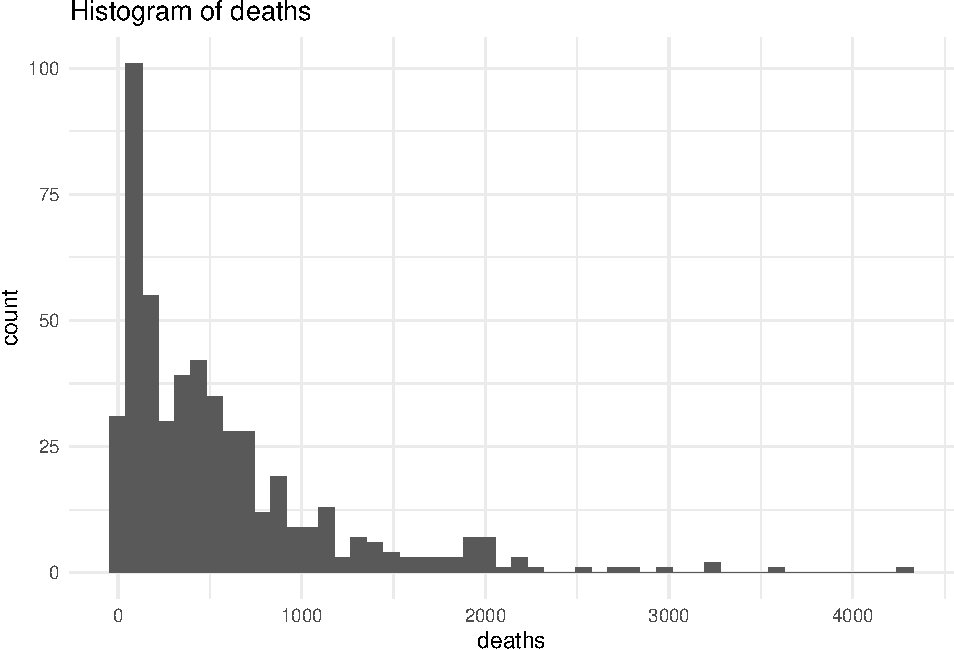
\includegraphics{Assignment_1_files/figure-latex/death distributions-1.pdf}

I can tell that the distribution is right-skewed and with quite some
observations out in the high deathcounts. This is without context so
next I wanna see if some particular states have large variations (of
course they do)

\begin{Shaded}
\begin{Highlighting}[]
\NormalTok{df }\OperatorTok\StringTok{ }\KeywordTok{ggplot}\NormalTok{() }\OperatorTok{+}
\StringTok{    }\KeywordTok{aes}\NormalTok{(}\DataTypeTok{x =}\NormalTok{ abbrev, }\DataTypeTok{y =}\NormalTok{ deaths) }\OperatorTok{+}
\StringTok{    }\KeywordTok{geom_violin}\NormalTok{() }\OperatorTok{+}
\StringTok{    }\CommentTok{# Stolen from your repo}
\StringTok{    }\KeywordTok{theme}\NormalTok{(}\DataTypeTok{axis.text.x =} \KeywordTok{element_text}\NormalTok{(}\DataTypeTok{angle =} \DecValTok{90}\NormalTok{, }\DataTypeTok{hjust =} \DecValTok{1}\NormalTok{, }\DataTypeTok{vjust =} \FloatTok{.5}\NormalTok{)) }\OperatorTok{+}
\StringTok{    }\KeywordTok{labs}\NormalTok{(}\DataTypeTok{title =} \StringTok{"Violin plots of deaths by state"}\NormalTok{)}
\end{Highlighting}
\end{Shaded}

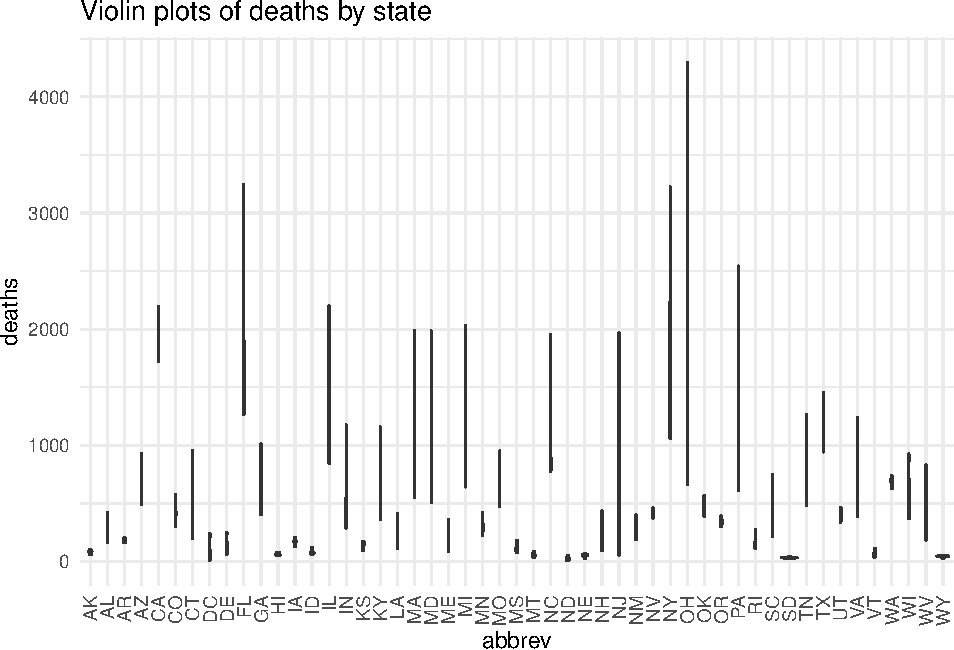
\includegraphics{Assignment_1_files/figure-latex/plots2-1.pdf}

There are a couple of states with huge variations like OH (Ohio?) or FL
(Florida) and quite a few of the states have very low variations and low
numbers. This is not as likely due to just population since California
would be somewhere in the sky. Next I'm gonna make sure that it's true
by looking at deaths vs pop and color the states.

\begin{Shaded}
\begin{Highlighting}[]
\NormalTok{df }\OperatorTok\StringTok{ }\KeywordTok{ggplot}\NormalTok{() }\OperatorTok{+}
\StringTok{    }\KeywordTok{aes}\NormalTok{(}\DataTypeTok{x =}\NormalTok{ total_pop, }\DataTypeTok{y =}\NormalTok{ deaths, }\DataTypeTok{color =}\NormalTok{ abbrev) }\OperatorTok{+}
\StringTok{    }\KeywordTok{geom_point}\NormalTok{() }\OperatorTok{+}
\StringTok{    }\KeywordTok{labs}\NormalTok{(}\DataTypeTok{title =} \StringTok{"Plot of deaths vs population by state"}\NormalTok{)}
\end{Highlighting}
\end{Shaded}

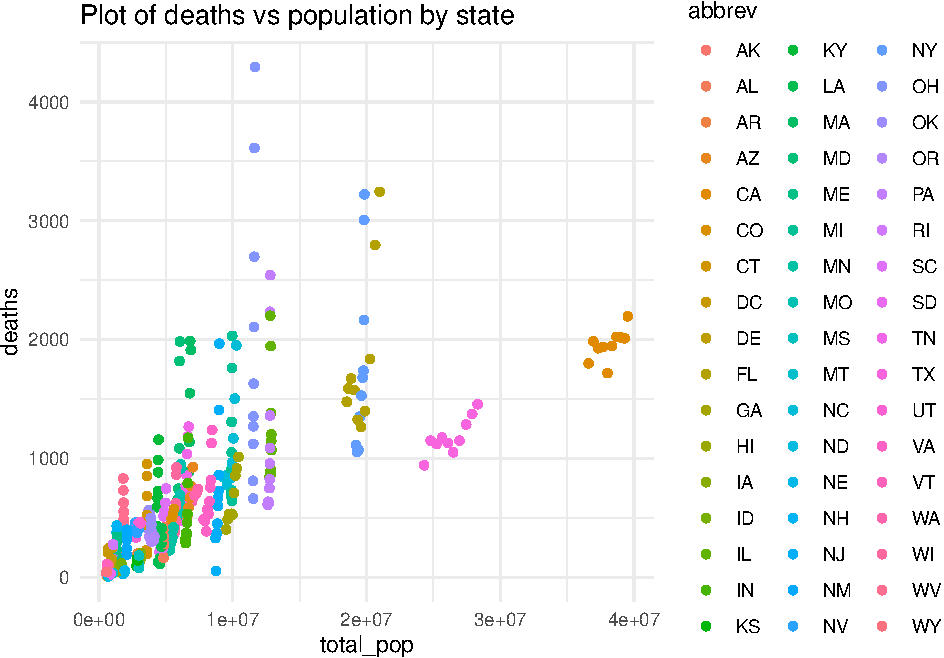
\includegraphics{Assignment_1_files/figure-latex/plots3-1.pdf}

There seems to be a population pattern to some degree (fair), but
overall there seems to be quite a lot of variation that's outside of
that. Let's look at mortality (deaths / pop) to see if there is
something a bit easier to spot.

\begin{Shaded}
\begin{Highlighting}[]
\NormalTok{df }\OperatorTok\StringTok{ }\KeywordTok{ggplot}\NormalTok{() }\OperatorTok{+}
\StringTok{    }\KeywordTok{aes}\NormalTok{(}\DataTypeTok{x =}\NormalTok{ abbrev, }\DataTypeTok{y =}\NormalTok{ deaths}\OperatorTok{/}\NormalTok{total_pop) }\OperatorTok{+}
\StringTok{    }\KeywordTok{geom_point}\NormalTok{() }\OperatorTok{+}
\StringTok{    }\KeywordTok{labs}\NormalTok{(}\DataTypeTok{title =} \StringTok{"Plot of mortality by state"}\NormalTok{) }\OperatorTok{+}
\StringTok{    }\KeywordTok{theme}\NormalTok{(}\DataTypeTok{axis.text.x =} \KeywordTok{element_text}\NormalTok{(}\DataTypeTok{angle =} \DecValTok{90}\NormalTok{, }\DataTypeTok{hjust =} \DecValTok{1}\NormalTok{, }\DataTypeTok{vjust =} \FloatTok{.5}\NormalTok{))}
\end{Highlighting}
\end{Shaded}

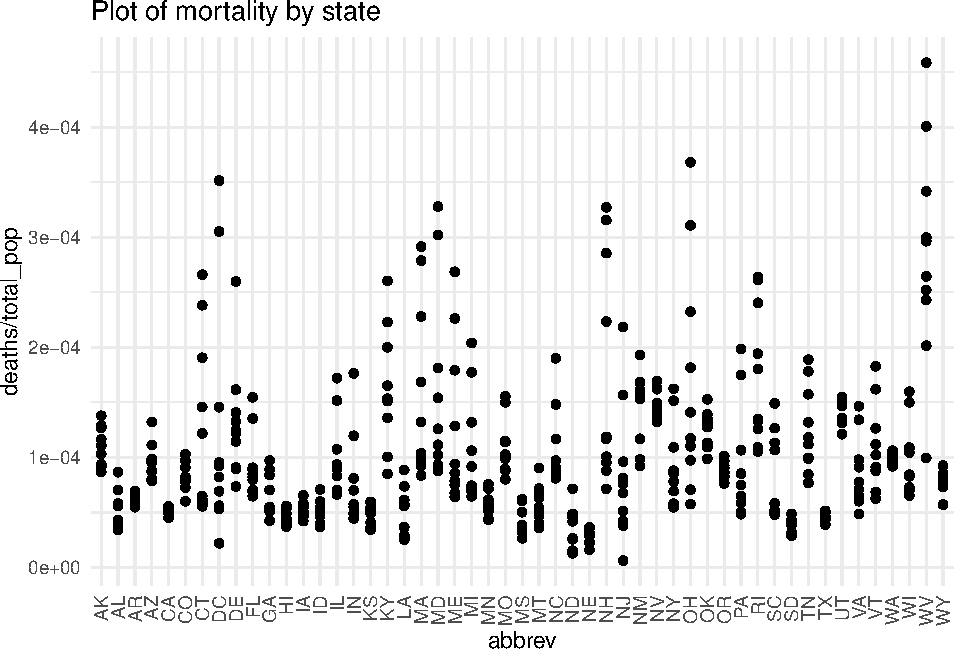
\includegraphics{Assignment_1_files/figure-latex/plots4-1.pdf}

This should show the variation in deaths that are not exactly just due
to high pop. Clearly there are some states that are way out there (again
OH). Let's check out the expected deaths vs actual

\begin{Shaded}
\begin{Highlighting}[]
\NormalTok{df }\OperatorTok\StringTok{ }\KeywordTok{ggplot}\NormalTok{() }\OperatorTok{+}
\StringTok{    }\KeywordTok{aes}\NormalTok{(}\DataTypeTok{x =}\NormalTok{ expected_deaths, }\DataTypeTok{y =}\NormalTok{ deaths) }\OperatorTok{+}
\StringTok{    }\KeywordTok{geom_point}\NormalTok{() }\OperatorTok{+}
\StringTok{    }\KeywordTok{labs}\NormalTok{(}\DataTypeTok{title =} \StringTok{"Plot of deaths vs expected deaths"}\NormalTok{)}
\end{Highlighting}
\end{Shaded}

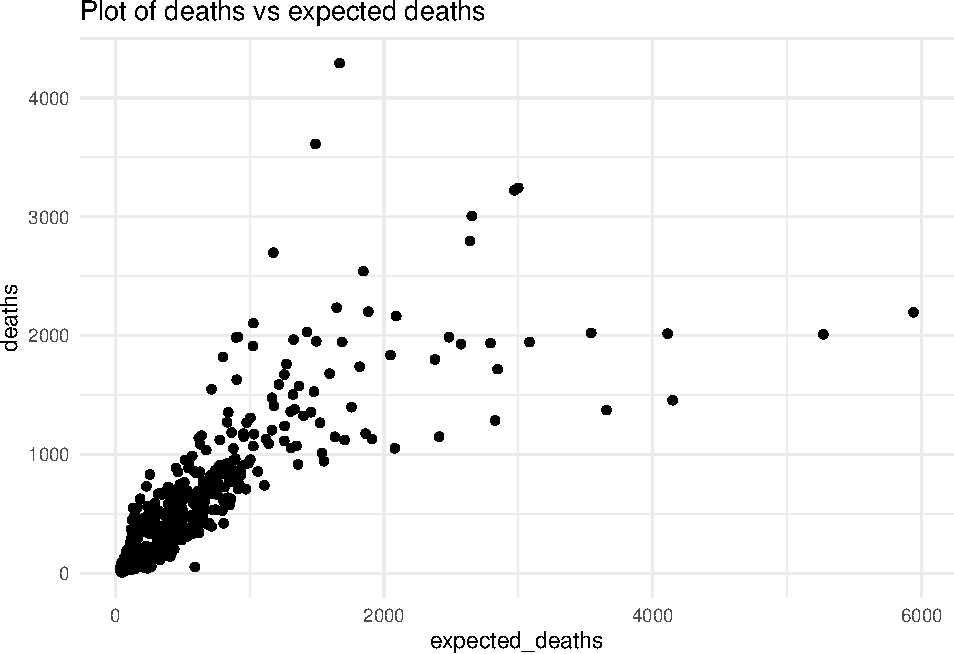
\includegraphics{Assignment_1_files/figure-latex/plots5-1.pdf}

This seems to make a lot better at predicting the actual deaths.
Probably a solid variable to use but by the data dictionary provided
it's a derivative of the other variables provided so probably unwise to
use it alongside them and make statements about those variables'
coefficients.

Let's check out whiteness

\begin{Shaded}
\begin{Highlighting}[]
\NormalTok{df }\OperatorTok\StringTok{ }\KeywordTok{ggplot}\NormalTok{() }\OperatorTok{+}
\StringTok{    }\KeywordTok{aes}\NormalTok{(}\DataTypeTok{x =}\NormalTok{ prop_white, }\DataTypeTok{y =}\NormalTok{ deaths) }\OperatorTok{+}
\StringTok{    }\KeywordTok{geom_point}\NormalTok{() }\OperatorTok{+}
\StringTok{    }\KeywordTok{labs}\NormalTok{(}\DataTypeTok{title =} \StringTok{"Plot of deaths vs proportion of white inhabitants"}\NormalTok{)}
\end{Highlighting}
\end{Shaded}

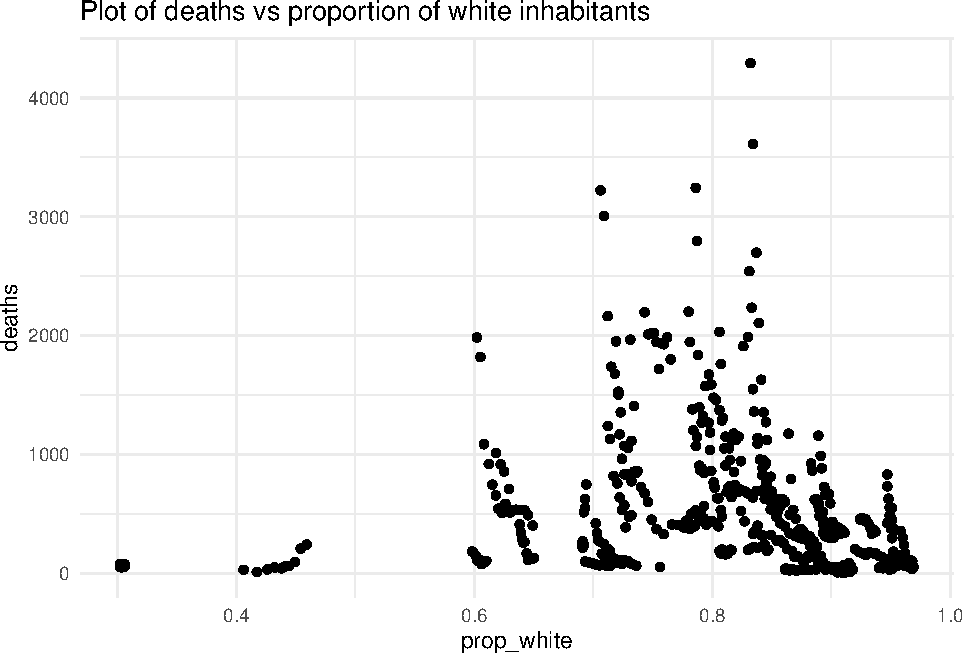
\includegraphics{Assignment_1_files/figure-latex/plots6-1.pdf}

This is a typical example of this:

\includegraphics{https://explainxkcd.com/wiki/images/9/91/linear_regression.png}

I don't think it's worth using it as a predictor. I could probably
massage this a bit and get something for the model but I highly doubt it
would have any real meaning. Let's check out prescription rates:

\begin{Shaded}
\begin{Highlighting}[]
\NormalTok{df }\OperatorTok\StringTok{ }\KeywordTok{ggplot}\NormalTok{() }\OperatorTok{+}
\StringTok{    }\KeywordTok{aes}\NormalTok{(}\DataTypeTok{x =}\NormalTok{ prescription_rate, }\DataTypeTok{y =}\NormalTok{ deaths) }\OperatorTok{+}
\StringTok{    }\KeywordTok{geom_point}\NormalTok{() }\OperatorTok{+}
\StringTok{    }\KeywordTok{labs}\NormalTok{(}\DataTypeTok{title =} \StringTok{"Plot of deaths vs prescription rate"}\NormalTok{)}
\end{Highlighting}
\end{Shaded}

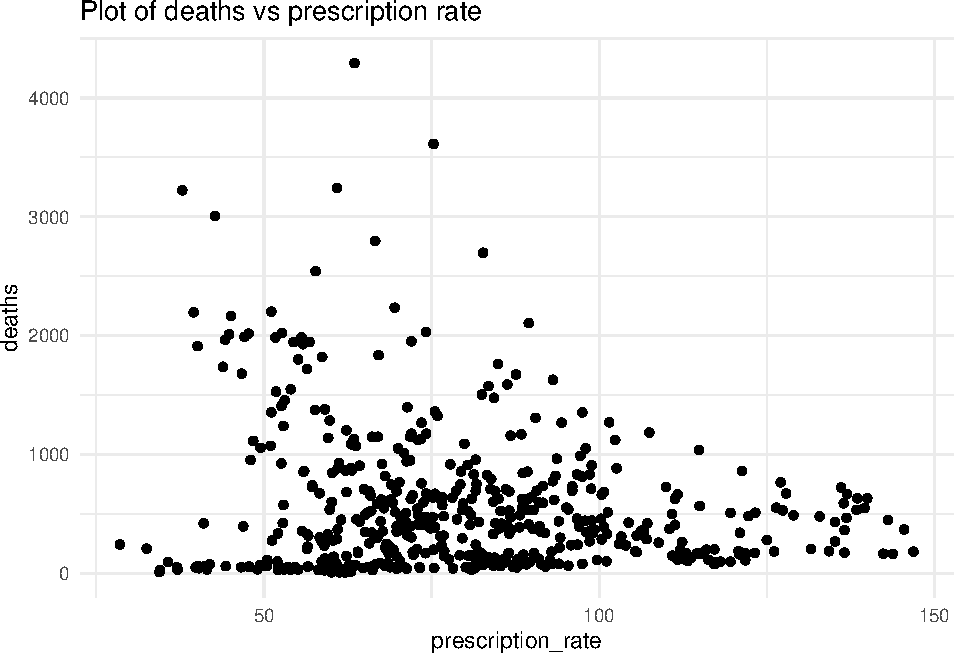
\includegraphics{Assignment_1_files/figure-latex/plots7-1.pdf}

Again there seems to be very minimal trend with overall prescription
rates. I don't think it's that good of a var. I could try to massage it
a bit by getting it to be prescription numbers

Finally let's take a look at the situation in the job market:

\begin{Shaded}
\begin{Highlighting}[]
\NormalTok{df }\OperatorTok\StringTok{ }\KeywordTok{ggplot}\NormalTok{() }\OperatorTok{+}
\StringTok{    }\KeywordTok{aes}\NormalTok{(}\DataTypeTok{x =}\NormalTok{ unemp, }\DataTypeTok{y =}\NormalTok{ deaths) }\OperatorTok{+}
\StringTok{    }\KeywordTok{geom_point}\NormalTok{() }\OperatorTok{+}
\StringTok{    }\KeywordTok{labs}\NormalTok{(}\DataTypeTok{title =} \StringTok{"Plot of deaths vs unemployment"}\NormalTok{)}
\end{Highlighting}
\end{Shaded}

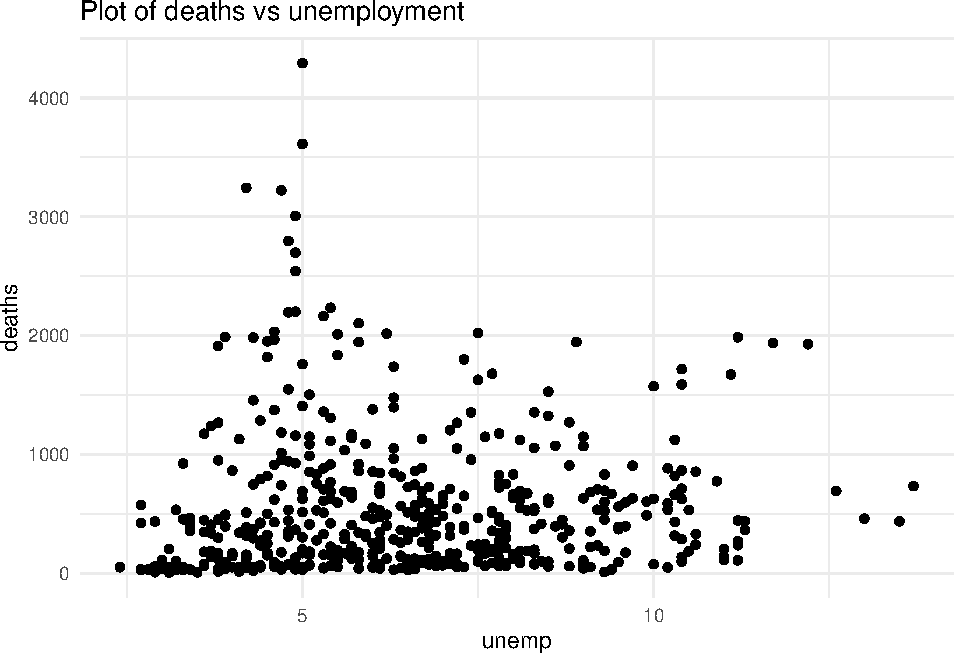
\includegraphics{Assignment_1_files/figure-latex/plots8-1.pdf}

Again there doesn't seem to be that much of a pattern. I don't know if
the variable is worthwhile to use.

Let's take a peek at the correlations

\begin{Shaded}
\begin{Highlighting}[]
\NormalTok{cor <-}\StringTok{ }\NormalTok{df }\OperatorTok\StringTok{ }\KeywordTok{select_if}\NormalTok{(is.numeric) }\OperatorTok\StringTok{ }\KeywordTok{cor}\NormalTok{()}

\KeywordTok{corrplot}\NormalTok{(cor, }\DataTypeTok{method =} \StringTok{"color"}\NormalTok{, }\DataTypeTok{type =} \StringTok{"lower"}\NormalTok{)}
\end{Highlighting}
\end{Shaded}

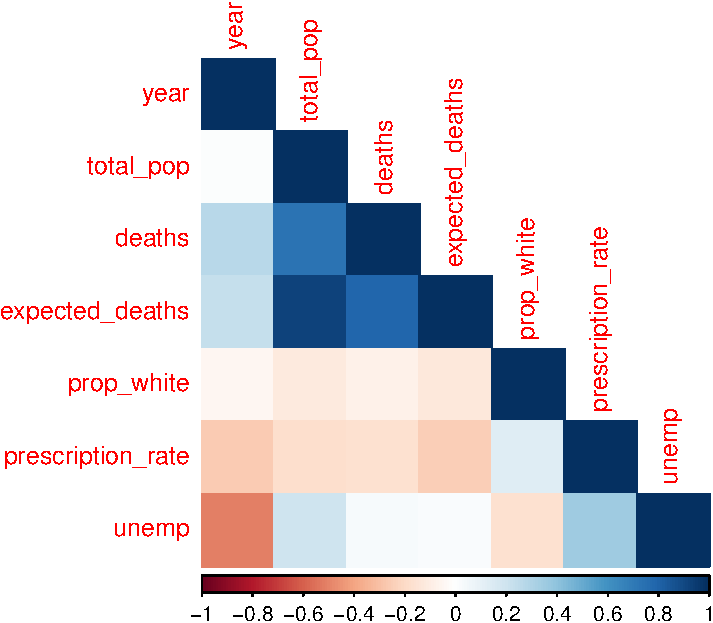
\includegraphics{Assignment_1_files/figure-latex/plots9-1.pdf}

\begin{Shaded}
\begin{Highlighting}[]
\NormalTok{summ_by_state <-}\StringTok{ }\NormalTok{df }\OperatorTok\StringTok{ }
\StringTok{    }\KeywordTok{mutate}\NormalTok{(}\DataTypeTok{mortality =}\NormalTok{ deaths}\OperatorTok{/}\NormalTok{total_pop) }\OperatorTok\StringTok{ }
\StringTok{    }\KeywordTok{group_by}\NormalTok{(state) }\OperatorTok
\StringTok{    }\KeywordTok{summarize}\NormalTok{(}\DataTypeTok{n =} \KeywordTok{n}\NormalTok{(),}
              \DataTypeTok{mean_deaths =} \KeywordTok{mean}\NormalTok{(deaths),}
              \DataTypeTok{var_deaths =} \KeywordTok{var}\NormalTok{(deaths),}
              \DataTypeTok{median_deaths =} \KeywordTok{median}\NormalTok{(deaths),}
              \DataTypeTok{min_deaths =} \KeywordTok{min}\NormalTok{(deaths),}
              \DataTypeTok{max_deaths =} \KeywordTok{max}\NormalTok{(deaths), }
              \DataTypeTok{mean_mort =} \KeywordTok{mean}\NormalTok{(mortality),}
              \DataTypeTok{var_mort =} \KeywordTok{var}\NormalTok{(mortality)}
\NormalTok{    )}
\end{Highlighting}
\end{Shaded}

\hypertarget{b-poisson-regression}{%
\subsection{b) Poisson Regression}\label{b-poisson-regression}}

\begin{Shaded}
\begin{Highlighting}[]
\NormalTok{df <-}\StringTok{ }\NormalTok{df }\OperatorTok\StringTok{ }\KeywordTok{mutate}\NormalTok{(}\DataTypeTok{state =} \KeywordTok{relevel}\NormalTok{(}\KeywordTok{as_factor}\NormalTok{(state),}\DataTypeTok{ref =} \StringTok{"Illinois"}\NormalTok{ ))}

\NormalTok{poiss_mod <-}\StringTok{ }\KeywordTok{glm}\NormalTok{(deaths}\OperatorTok{~}\StringTok{ }\NormalTok{state }\OperatorTok{+}\StringTok{ }\NormalTok{expected_deaths }\OperatorTok{+}\StringTok{ }\NormalTok{prescription_rate, }\DataTypeTok{family =}\NormalTok{ poisson, }\DataTypeTok{data =}\NormalTok{ df, }\DataTypeTok{offset =} \KeywordTok{log}\NormalTok{(total_pop))}

\KeywordTok{summary}\NormalTok{(poiss_mod)}
\end{Highlighting}
\end{Shaded}

\begin{verbatim}
## 
## Call:
## glm(formula = deaths ~ state + expected_deaths + prescription_rate, 
##     family = poisson, data = df, offset = log(total_pop))
## 
## Deviance Residuals: 
##      Min        1Q    Median        3Q       Max  
## -30.6815   -3.1970   -0.0585    2.7924   24.5650  
## 
## Coefficients:
##                             Estimate Std. Error  z value Pr(>|z|)    
## (Intercept)               -7.982e+00  1.993e-02 -400.423  < 2e-16 ***
## stateAlabama               1.002e+00  2.634e-02   38.053  < 2e-16 ***
## stateAlaska                3.427e-01  3.650e-02    9.389  < 2e-16 ***
## stateArizona               4.603e-01  1.581e-02   29.120  < 2e-16 ***
## stateArkansas              9.480e-01  2.746e-02   34.519  < 2e-16 ***
## stateCalifornia           -1.159e+00  1.591e-02  -72.850  < 2e-16 ***
## stateColorado              8.653e-02  1.766e-02    4.899 9.65e-07 ***
## stateConnecticut           4.406e-01  1.771e-02   24.883  < 2e-16 ***
## stateDelaware              1.094e+00  3.051e-02   35.856  < 2e-16 ***
## stateDistrict of Columbia -1.200e-01  3.678e-02   -3.261  0.00111 ** 
## stateFlorida               1.920e-01  1.290e-02   14.886  < 2e-16 ***
## stateGeorgia               1.657e-01  1.600e-02   10.354  < 2e-16 ***
## stateHawaii               -9.469e-01  4.110e-02  -23.040  < 2e-16 ***
## stateIdaho                 1.346e-02  3.645e-02    0.369  0.71197    
## stateIndiana               6.538e-01  1.812e-02   36.071  < 2e-16 ***
## stateIowa                 -3.820e-01  2.644e-02  -14.447  < 2e-16 ***
## stateKansas               -6.140e-02  2.846e-02   -2.157  0.03099 *  
## stateKentucky              1.848e+00  1.794e-02  103.039  < 2e-16 ***
## stateLouisiana             4.569e-01  2.470e-02   18.501  < 2e-16 ***
## stateMaine                 8.490e-01  2.628e-02   32.304  < 2e-16 ***
## stateMaryland              6.775e-01  1.389e-02   48.790  < 2e-16 ***
## stateMassachusetts         5.140e-01  1.352e-02   38.018  < 2e-16 ***
## stateMichigan              8.400e-01  1.473e-02   57.031  < 2e-16 ***
## stateMinnesota            -5.901e-01  2.053e-02  -28.744  < 2e-16 ***
## stateMississippi           4.470e-01  3.165e-02   14.122  < 2e-16 ***
## stateMissouri              8.029e-01  1.602e-02   50.135  < 2e-16 ***
## stateMontana               2.001e-02  4.287e-02    0.467  0.64076    
## stateNebraska             -9.933e-01  4.519e-02  -21.980  < 2e-16 ***
## stateNevada                1.215e+00  1.866e-02   65.097  < 2e-16 ***
## stateNew Hampshire         1.050e+00  2.297e-02   45.711  < 2e-16 ***
## stateNew Jersey           -1.931e-01  1.482e-02  -13.029  < 2e-16 ***
## stateNew Mexico            7.827e-01  2.060e-02   37.992  < 2e-16 ***
## stateNew York             -4.635e-01  1.204e-02  -38.503  < 2e-16 ***
## stateNorth Carolina        7.870e-01  1.447e-02   54.375  < 2e-16 ***
## stateNorth Dakota         -9.832e-01  6.402e-02  -15.356  < 2e-16 ***
## stateOhio                  1.206e+00  1.285e-02   93.851  < 2e-16 ***
## stateOklahoma              1.496e+00  1.953e-02   76.630  < 2e-16 ***
## stateOregon                6.475e-01  1.998e-02   32.414  < 2e-16 ***
## statePennsylvania          2.906e-01  1.333e-02   21.796  < 2e-16 ***
## stateRhode Island          9.966e-01  2.528e-02   39.427  < 2e-16 ***
## stateSouth Carolina        7.143e-01  1.951e-02   36.620  < 2e-16 ***
## stateSouth Dakota         -8.878e-01  5.633e-02  -15.761  < 2e-16 ***
## stateTennessee             1.742e+00  1.893e-02   92.025  < 2e-16 ***
## stateTexas                -8.110e-01  1.477e-02  -54.915  < 2e-16 ***
## stateUtah                  9.276e-01  1.840e-02   50.417  < 2e-16 ***
## stateVermont               1.022e-01  3.994e-02    2.560  0.01048 *  
## stateVirginia              1.551e-01  1.501e-02   10.329  < 2e-16 ***
## stateWashington            3.995e-01  1.524e-02   26.221  < 2e-16 ***
## stateWest Virginia         2.567e+00  1.948e-02  131.762  < 2e-16 ***
## stateWisconsin             3.126e-01  1.611e-02   19.407  < 2e-16 ***
## stateWyoming               3.095e-01  4.808e-02    6.437 1.22e-10 ***
## expected_deaths            1.186e-04  4.565e-06   25.980  < 2e-16 ***
## prescription_rate         -2.310e-02  2.338e-04  -98.808  < 2e-16 ***
## ---
## Signif. codes:  0 '***' 0.001 '**' 0.01 '*' 0.05 '.' 0.1 ' ' 1
## 
## (Dispersion parameter for poisson family taken to be 1)
## 
##     Null deviance: 87495  on 509  degrees of freedom
## Residual deviance: 18875  on 457  degrees of freedom
## AIC: 22843
## 
## Number of Fisher Scoring iterations: 4
\end{verbatim}

\begin{Shaded}
\begin{Highlighting}[]
\NormalTok{GGally}\OperatorTok{::}\KeywordTok{ggcoef}\NormalTok{(poiss_mod, }\DataTypeTok{exponentiate =} \OtherTok{TRUE}\NormalTok{)}
\end{Highlighting}
\end{Shaded}

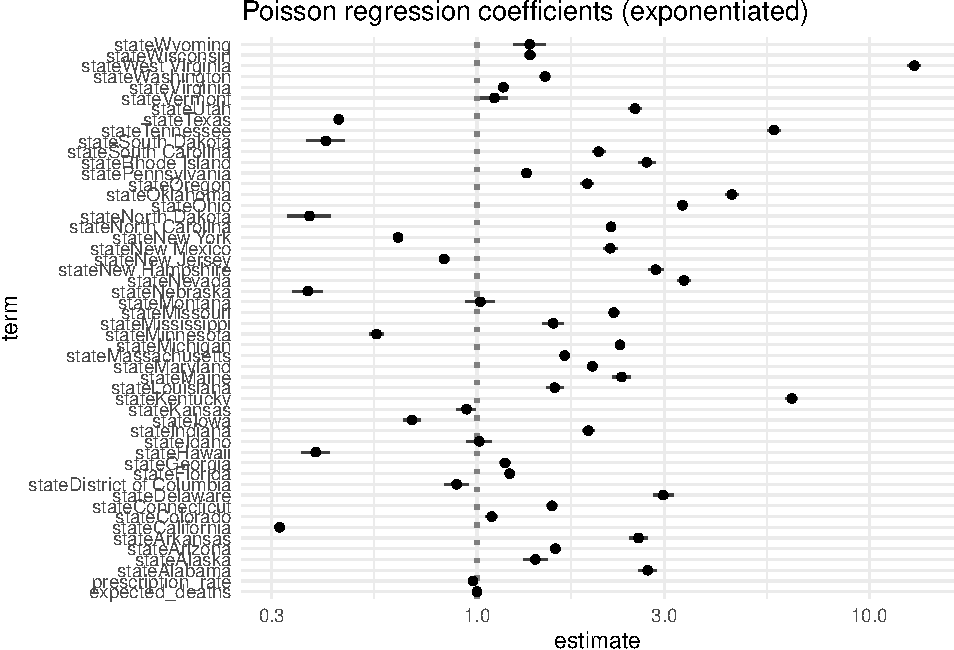
\includegraphics{Assignment_1_files/figure-latex/visualizing poiss reg-1.pdf}

\hypertarget{c-population-offset}{%
\subsection{c) Population offset}\label{c-population-offset}}

by the hint - population age distribution (as well as other possible
confounds) are not accounted for - old people in Florida probably die a
lot more than the youth in Washington.

\hypertarget{d-poisson-regression---expected_deaths}{%
\subsection{d) Poisson Regression -
expected\_deaths}\label{d-poisson-regression---expected_deaths}}

\begin{Shaded}
\begin{Highlighting}[]
\NormalTok{poiss_mod2 <-}\StringTok{ }\KeywordTok{glm}\NormalTok{(deaths}\OperatorTok{~}\StringTok{ }\NormalTok{state }\OperatorTok{+}\StringTok{ }\NormalTok{prescription_rate, }\DataTypeTok{family =}\NormalTok{ poisson, }\DataTypeTok{data =}\NormalTok{ df, }\DataTypeTok{offset =} \KeywordTok{log}\NormalTok{(expected_deaths))}

\KeywordTok{summary}\NormalTok{(poiss_mod2)}
\end{Highlighting}
\end{Shaded}

\begin{verbatim}
## 
## Call:
## glm(formula = deaths ~ state + prescription_rate, family = poisson, 
##     data = df, offset = log(expected_deaths))
## 
## Deviance Residuals: 
##      Min        1Q    Median        3Q       Max  
## -27.0082   -2.4650    0.0442    2.4398   19.0997  
## 
## Coefficients:
##                             Estimate Std. Error z value Pr(>|z|)    
## (Intercept)                0.1151819  0.0144904   7.949 1.88e-15 ***
## stateAlabama              -0.6031519  0.0257873 -23.390  < 2e-16 ***
## stateAlaska                0.1097643  0.0361794   3.034 0.002414 ** 
## stateArizona               0.0255170  0.0158007   1.615 0.106327    
## stateArkansas             -0.3801609  0.0272811 -13.935  < 2e-16 ***
## stateCalifornia           -0.6630030  0.0116098 -57.107  < 2e-16 ***
## stateColorado             -0.1692181  0.0175128  -9.663  < 2e-16 ***
## stateConnecticut           0.2703020  0.0173465  15.582  < 2e-16 ***
## stateDelaware              0.3371956  0.0304757  11.064  < 2e-16 ***
## stateDistrict of Columbia  0.1567998  0.0358090   4.379 1.19e-05 ***
## stateFlorida              -0.0204810  0.0118968  -1.722 0.085149 .  
## stateGeorgia              -0.3886990  0.0158693 -24.494  < 2e-16 ***
## stateHawaii               -0.7515957  0.0405336 -18.543  < 2e-16 ***
## stateIdaho                -0.5888151  0.0364016 -16.176  < 2e-16 ***
## stateIndiana              -0.2011187  0.0180568 -11.138  < 2e-16 ***
## stateIowa                 -0.5500446  0.0261881 -21.004  < 2e-16 ***
## stateKansas               -0.6343163  0.0284258 -22.315  < 2e-16 ***
## stateKentucky              0.5643082  0.0179581  31.424  < 2e-16 ***
## stateLouisiana            -0.6573303  0.0245382 -26.788  < 2e-16 ***
## stateMaine                 0.2902132  0.0261828  11.084  < 2e-16 ***
## stateMaryland              0.4758297  0.0136975  34.738  < 2e-16 ***
## stateMassachusetts         0.4677374  0.0132250  35.368  < 2e-16 ***
## stateMichigan              0.1311816  0.0144749   9.063  < 2e-16 ***
## stateMinnesota            -0.5309103  0.0201383 -26.363  < 2e-16 ***
## stateMississippi          -0.7952790  0.0315354 -25.219  < 2e-16 ***
## stateMissouri              0.1570852  0.0159997   9.818  < 2e-16 ***
## stateMontana              -0.4973615  0.0427850 -11.625  < 2e-16 ***
## stateNebraska             -1.2184855  0.0450237 -27.063  < 2e-16 ***
## stateNevada                0.4357719  0.0186464  23.370  < 2e-16 ***
## stateNew Hampshire         0.5847623  0.0227720  25.679  < 2e-16 ***
## stateNew Jersey           -0.1555337  0.0146629 -10.607  < 2e-16 ***
## stateNew Mexico            0.4560740  0.0203480  22.414  < 2e-16 ***
## stateNew York             -0.0861113  0.0119674  -7.195 6.22e-13 ***
## stateNorth Carolina        0.1223722  0.0142583   8.583  < 2e-16 ***
## stateNorth Dakota         -1.0126553  0.0637594 -15.882  < 2e-16 ***
## stateOhio                  0.5934686  0.0125560  47.266  < 2e-16 ***
## stateOklahoma              0.3109461  0.0194118  16.018  < 2e-16 ***
## stateOregon               -0.0963428  0.0200004  -4.817 1.46e-06 ***
## statePennsylvania         -0.0355564  0.0131935  -2.695 0.007039 ** 
## stateRhode Island          0.5918762  0.0250275  23.649  < 2e-16 ***
## stateSouth Carolina       -0.1364762  0.0194754  -7.008 2.42e-12 ***
## stateSouth Dakota         -0.8681808  0.0560265 -15.496  < 2e-16 ***
## stateTennessee             0.3000179  0.0183596  16.341  < 2e-16 ***
## stateTexas                -0.7683252  0.0128625 -59.734  < 2e-16 ***
## stateUtah                  0.4476126  0.0182937  24.468  < 2e-16 ***
## stateVermont               0.1168908  0.0394756   2.961 0.003066 ** 
## stateVirginia             -0.1361692  0.0150069  -9.074  < 2e-16 ***
## stateWashington            0.0028164  0.0152289   0.185 0.853279    
## stateWest Virginia         1.1421947  0.0199774  57.174  < 2e-16 ***
## stateWisconsin             0.0565688  0.0159898   3.538 0.000403 ***
## stateWyoming              -0.1844081  0.0479815  -3.843 0.000121 ***
## prescription_rate         -0.0006780  0.0001908  -3.554 0.000379 ***
## ---
## Signif. codes:  0 '***' 0.001 '**' 0.01 '*' 0.05 '.' 0.1 ' ' 1
## 
## (Dispersion parameter for poisson family taken to be 1)
## 
##     Null deviance: 63933  on 509  degrees of freedom
## Residual deviance: 13675  on 458  degrees of freedom
## AIC: 17641
## 
## Number of Fisher Scoring iterations: 4
\end{verbatim}

\hypertarget{e-overdispersion}{%
\subsection{e) Overdispersion}\label{e-overdispersion}}

\begin{Shaded}
\begin{Highlighting}[]
\NormalTok{res <-}\StringTok{ }\NormalTok{df }\OperatorTok
\StringTok{    }\KeywordTok{mutate}\NormalTok{(}\DataTypeTok{predictions =} \KeywordTok{predict}\NormalTok{(poiss_mod2, }\DataTypeTok{newdata =}\NormalTok{ df, }\DataTypeTok{type =} \StringTok{"response"}\NormalTok{)) }\OperatorTok
\StringTok{    }\KeywordTok{select}\NormalTok{(deaths, predictions) }\OperatorTok
\StringTok{    }\KeywordTok{mutate}\NormalTok{(}\DataTypeTok{residuals =}\NormalTok{ deaths }\OperatorTok{-}\StringTok{ }\NormalTok{predictions,}
           \DataTypeTok{z =}\NormalTok{ residuals }\OperatorTok{/}\StringTok{ }\KeywordTok{sd}\NormalTok{(predictions))}

\NormalTok{res }\OperatorTok
\StringTok{    }\KeywordTok{ggplot}\NormalTok{() }\OperatorTok{+}
\StringTok{    }\KeywordTok{aes}\NormalTok{(}\DataTypeTok{x =}\NormalTok{ deaths,}
        \DataTypeTok{y =}\NormalTok{ residuals) }\OperatorTok{+}
\StringTok{    }\KeywordTok{geom_point}\NormalTok{() }\OperatorTok{+}
\StringTok{    }\KeywordTok{geom_abline}\NormalTok{(}\DataTypeTok{slope =} \DecValTok{1}\NormalTok{,}
                \DataTypeTok{intercept =} \DecValTok{0}\NormalTok{,}
                \DataTypeTok{color =} \StringTok{"red"}\NormalTok{) }\OperatorTok{+}
\StringTok{    }\KeywordTok{geom_abline}\NormalTok{(}\DataTypeTok{slope =} \DecValTok{-1}\NormalTok{,}
                \DataTypeTok{intercept =} \DecValTok{0}\NormalTok{,}
                \DataTypeTok{color =} \StringTok{"red"}\NormalTok{)}
\end{Highlighting}
\end{Shaded}

\includegraphics{Assignment_1_files/figure-latex/overdispersion-1.pdf}

\begin{Shaded}
\begin{Highlighting}[]
\NormalTok{res_summary <-}\StringTok{ }\NormalTok{res }\OperatorTok
\StringTok{    }\KeywordTok{summarize}\NormalTok{(}\DataTypeTok{mean =} \KeywordTok{mean}\NormalTok{(z),}
              \DataTypeTok{sd =} \KeywordTok{sd}\NormalTok{(z))}

\NormalTok{res_summary }\OperatorTok\StringTok{ }\NormalTok{kableExtra}\OperatorTok{::}\KeywordTok{kable}\NormalTok{()}
\end{Highlighting}
\end{Shaded}

\begin{tabular}{r|r}
\hline
mean & sd\\
\hline
0 & 0.29287\\
\hline
\end{tabular}

Estimated overdispersion factor:

\begin{Shaded}
\begin{Highlighting}[]
\CommentTok{# Doesn't work for some ungodly reason}
\CommentTok{# n <- length(df$year)}
\CommentTok{# k <- length(coef(poiss_mod2))}
\CommentTok{# }
\CommentTok{# overdisp_factor1 <- sum(res$z^2) / (n - k)}

\NormalTok{qusipoiss_mod <-}\StringTok{ }\KeywordTok{glm}\NormalTok{(deaths}\OperatorTok{~}\StringTok{ }\NormalTok{state }\OperatorTok{+}\StringTok{ }\NormalTok{expected_deaths }\OperatorTok{+}\StringTok{ }\NormalTok{prescription_rate, }\DataTypeTok{family =}\NormalTok{ quasipoisson, }\DataTypeTok{data =}\NormalTok{ df, }\DataTypeTok{offset =} \KeywordTok{log}\NormalTok{(expected_deaths))}

\NormalTok{overdisp_factor <-}\StringTok{ }\KeywordTok{summary}\NormalTok{(qusipoiss_mod)}\OperatorTok{$}\NormalTok{dispersion}
\end{Highlighting}
\end{Shaded}

\hypertarget{f-neg-bin-regression}{%
\subsection{f) Neg Bin Regression}\label{f-neg-bin-regression}}

\begin{Shaded}
\begin{Highlighting}[]
\NormalTok{neg_bin_mod <-}\StringTok{ }\NormalTok{MASS}\OperatorTok{::}\KeywordTok{glm.nb}\NormalTok{(deaths}\OperatorTok{~}\StringTok{ }\NormalTok{state }\OperatorTok{+}\StringTok{ }\NormalTok{prescription_rate, }\DataTypeTok{data =}\NormalTok{ df)}
\KeywordTok{summary}\NormalTok{(neg_bin_mod)}
\end{Highlighting}
\end{Shaded}

\begin{verbatim}
## 
## Call:
## MASS::glm.nb(formula = deaths ~ state + prescription_rate, data = df, 
##     init.theta = 13.68097651, link = log)
## 
## Deviance Residuals: 
##     Min       1Q   Median       3Q      Max  
## -6.3034  -0.6744  -0.0597   0.5297   3.7426  
## 
## Coefficients:
##                            Estimate Std. Error z value Pr(>|z|)    
## (Intercept)                8.646336   0.121693  71.051  < 2e-16 ***
## stateAlabama               0.102352   0.157561   0.650 0.515948    
## stateAlaska               -2.634616   0.126329 -20.855  < 2e-16 ***
## stateArizona              -0.195272   0.124755  -1.565 0.117525    
## stateArkansas             -0.476785   0.146738  -3.249 0.001157 ** 
## stateCalifornia            0.250149   0.122126   2.048 0.040532 *  
## stateColorado             -0.846953   0.122558  -6.911 4.82e-12 ***
## stateConnecticut          -0.971749   0.122341  -7.943 1.97e-15 ***
## stateDelaware             -1.599969   0.131572 -12.160  < 2e-16 ***
## stateDistrict of Columbia -3.330655   0.130924 -25.440  < 2e-16 ***
## stateFlorida               0.759922   0.123315   6.162 7.16e-10 ***
## stateGeorgia              -0.058786   0.126312  -0.465 0.641645    
## stateHawaii               -3.294614   0.129081 -25.524  < 2e-16 ***
## stateIdaho                -2.108554   0.130702 -16.133  < 2e-16 ***
## stateIndiana              -0.031113   0.133238  -0.234 0.815363    
## stateIowa                 -1.868482   0.123877 -15.083  < 2e-16 ***
## stateKansas               -1.575975   0.128122 -12.301  < 2e-16 ***
## stateKentucky              0.900625   0.146418   6.151 7.70e-10 ***
## stateLouisiana            -0.569071   0.139719  -4.073 4.64e-05 ***
## stateMaine                -1.539412   0.127517 -12.072  < 2e-16 ***
## stateMaryland             -0.193799   0.121936  -1.589 0.111980    
## stateMassachusetts        -0.238689   0.121687  -1.962 0.049820 *  
## stateMichigan              0.610718   0.129631   4.711 2.46e-06 ***
## stateMinnesota            -1.530105   0.122884 -12.452  < 2e-16 ***
## stateMississippi          -0.990979   0.145132  -6.828 8.60e-12 ***
## stateMissouri              0.050460   0.127592   0.395 0.692486    
## stateMontana              -2.523458   0.130810 -19.291  < 2e-16 ***
## stateNebraska             -3.004593   0.129327 -23.232  < 2e-16 ***
## stateNevada               -0.278294   0.129391  -2.151 0.031492 *  
## stateNew Hampshire        -1.339690   0.125117 -10.708  < 2e-16 ***
## stateNew Jersey           -0.656946   0.121962  -5.386 7.19e-08 ***
## stateNew Mexico           -1.110893   0.123676  -8.982  < 2e-16 ***
## stateNew York              0.001962   0.123090   0.016 0.987281    
## stateNorth Carolina        0.553997   0.128351   4.316 1.59e-05 ***
## stateNorth Dakota         -4.018679   0.137475 -29.232  < 2e-16 ***
## stateOhio                  1.105209   0.128512   8.600  < 2e-16 ***
## stateOklahoma              0.425805   0.142006   2.998 0.002713 ** 
## stateOregon               -0.454757   0.129751  -3.505 0.000457 ***
## statePennsylvania          0.287386   0.123652   2.324 0.020117 *  
## stateRhode Island         -1.595766   0.125028 -12.763  < 2e-16 ***
## stateSouth Carolina       -0.290666   0.131998  -2.202 0.027662 *  
## stateSouth Dakota         -3.742793   0.133501 -28.036  < 2e-16 ***
## stateTennessee             1.191926   0.152092   7.837 4.62e-15 ***
## stateTexas                 0.126622   0.121912   1.039 0.298973    
## stateUtah                 -0.584797   0.125376  -4.664 3.10e-06 ***
## stateVermont              -3.044833   0.127501 -23.881  < 2e-16 ***
## stateVirginia             -0.319654   0.122780  -2.603 0.009228 ** 
## stateWashington           -0.165792   0.123722  -1.340 0.180232    
## stateWest Virginia         0.791776   0.152631   5.188 2.13e-07 ***
## stateWisconsin            -0.546001   0.122641  -4.452 8.51e-06 ***
## stateWyoming              -2.867325   0.132180 -21.693  < 2e-16 ***
## prescription_rate         -0.025378   0.001417 -17.906  < 2e-16 ***
## ---
## Signif. codes:  0 '***' 0.001 '**' 0.01 '*' 0.05 '.' 0.1 ' ' 1
## 
## (Dispersion parameter for Negative Binomial(13.681) family taken to be 1)
## 
##     Null deviance: 7771.13  on 509  degrees of freedom
## Residual deviance:  519.94  on 458  degrees of freedom
## AIC: 6125.7
## 
## Number of Fisher Scoring iterations: 1
## 
## 
##               Theta:  13.681 
##           Std. Err.:  0.914 
## 
##  2 x log-likelihood:  -6019.675
\end{verbatim}

\hypertarget{g-summary}{%
\subsection{g) Summary}\label{g-summary}}

\end{document}
